% Options for packages loaded elsewhere
\PassOptionsToPackage{unicode}{hyperref}
\PassOptionsToPackage{hyphens}{url}
%
\documentclass[
]{article}
\usepackage{amsmath,amssymb}
\usepackage{lmodern}
\usepackage{iftex}
\ifPDFTeX
  \usepackage[T1]{fontenc}
  \usepackage[utf8]{inputenc}
  \usepackage{textcomp} % provide euro and other symbols
\else % if luatex or xetex
  \usepackage{unicode-math}
  \defaultfontfeatures{Scale=MatchLowercase}
  \defaultfontfeatures[\rmfamily]{Ligatures=TeX,Scale=1}
\fi
% Use upquote if available, for straight quotes in verbatim environments
\IfFileExists{upquote.sty}{\usepackage{upquote}}{}
\IfFileExists{microtype.sty}{% use microtype if available
  \usepackage[]{microtype}
  \UseMicrotypeSet[protrusion]{basicmath} % disable protrusion for tt fonts
}{}
\makeatletter
\@ifundefined{KOMAClassName}{% if non-KOMA class
  \IfFileExists{parskip.sty}{%
    \usepackage{parskip}
  }{% else
    \setlength{\parindent}{0pt}
    \setlength{\parskip}{6pt plus 2pt minus 1pt}}
}{% if KOMA class
  \KOMAoptions{parskip=half}}
\makeatother
\usepackage{xcolor}
\IfFileExists{xurl.sty}{\usepackage{xurl}}{} % add URL line breaks if available
\IfFileExists{bookmark.sty}{\usepackage{bookmark}}{\usepackage{hyperref}}
\hypersetup{
  pdftitle={DatosAgrupados},
  pdfauthor={Gabriel},
  hidelinks,
  pdfcreator={LaTeX via pandoc}}
\urlstyle{same} % disable monospaced font for URLs
\usepackage[margin=1in]{geometry}
\usepackage{color}
\usepackage{fancyvrb}
\newcommand{\VerbBar}{|}
\newcommand{\VERB}{\Verb[commandchars=\\\{\}]}
\DefineVerbatimEnvironment{Highlighting}{Verbatim}{commandchars=\\\{\}}
% Add ',fontsize=\small' for more characters per line
\usepackage{framed}
\definecolor{shadecolor}{RGB}{248,248,248}
\newenvironment{Shaded}{\begin{snugshade}}{\end{snugshade}}
\newcommand{\AlertTok}[1]{\textcolor[rgb]{0.94,0.16,0.16}{#1}}
\newcommand{\AnnotationTok}[1]{\textcolor[rgb]{0.56,0.35,0.01}{\textbf{\textit{#1}}}}
\newcommand{\AttributeTok}[1]{\textcolor[rgb]{0.77,0.63,0.00}{#1}}
\newcommand{\BaseNTok}[1]{\textcolor[rgb]{0.00,0.00,0.81}{#1}}
\newcommand{\BuiltInTok}[1]{#1}
\newcommand{\CharTok}[1]{\textcolor[rgb]{0.31,0.60,0.02}{#1}}
\newcommand{\CommentTok}[1]{\textcolor[rgb]{0.56,0.35,0.01}{\textit{#1}}}
\newcommand{\CommentVarTok}[1]{\textcolor[rgb]{0.56,0.35,0.01}{\textbf{\textit{#1}}}}
\newcommand{\ConstantTok}[1]{\textcolor[rgb]{0.00,0.00,0.00}{#1}}
\newcommand{\ControlFlowTok}[1]{\textcolor[rgb]{0.13,0.29,0.53}{\textbf{#1}}}
\newcommand{\DataTypeTok}[1]{\textcolor[rgb]{0.13,0.29,0.53}{#1}}
\newcommand{\DecValTok}[1]{\textcolor[rgb]{0.00,0.00,0.81}{#1}}
\newcommand{\DocumentationTok}[1]{\textcolor[rgb]{0.56,0.35,0.01}{\textbf{\textit{#1}}}}
\newcommand{\ErrorTok}[1]{\textcolor[rgb]{0.64,0.00,0.00}{\textbf{#1}}}
\newcommand{\ExtensionTok}[1]{#1}
\newcommand{\FloatTok}[1]{\textcolor[rgb]{0.00,0.00,0.81}{#1}}
\newcommand{\FunctionTok}[1]{\textcolor[rgb]{0.00,0.00,0.00}{#1}}
\newcommand{\ImportTok}[1]{#1}
\newcommand{\InformationTok}[1]{\textcolor[rgb]{0.56,0.35,0.01}{\textbf{\textit{#1}}}}
\newcommand{\KeywordTok}[1]{\textcolor[rgb]{0.13,0.29,0.53}{\textbf{#1}}}
\newcommand{\NormalTok}[1]{#1}
\newcommand{\OperatorTok}[1]{\textcolor[rgb]{0.81,0.36,0.00}{\textbf{#1}}}
\newcommand{\OtherTok}[1]{\textcolor[rgb]{0.56,0.35,0.01}{#1}}
\newcommand{\PreprocessorTok}[1]{\textcolor[rgb]{0.56,0.35,0.01}{\textit{#1}}}
\newcommand{\RegionMarkerTok}[1]{#1}
\newcommand{\SpecialCharTok}[1]{\textcolor[rgb]{0.00,0.00,0.00}{#1}}
\newcommand{\SpecialStringTok}[1]{\textcolor[rgb]{0.31,0.60,0.02}{#1}}
\newcommand{\StringTok}[1]{\textcolor[rgb]{0.31,0.60,0.02}{#1}}
\newcommand{\VariableTok}[1]{\textcolor[rgb]{0.00,0.00,0.00}{#1}}
\newcommand{\VerbatimStringTok}[1]{\textcolor[rgb]{0.31,0.60,0.02}{#1}}
\newcommand{\WarningTok}[1]{\textcolor[rgb]{0.56,0.35,0.01}{\textbf{\textit{#1}}}}
\usepackage{graphicx}
\makeatletter
\def\maxwidth{\ifdim\Gin@nat@width>\linewidth\linewidth\else\Gin@nat@width\fi}
\def\maxheight{\ifdim\Gin@nat@height>\textheight\textheight\else\Gin@nat@height\fi}
\makeatother
% Scale images if necessary, so that they will not overflow the page
% margins by default, and it is still possible to overwrite the defaults
% using explicit options in \includegraphics[width, height, ...]{}
\setkeys{Gin}{width=\maxwidth,height=\maxheight,keepaspectratio}
% Set default figure placement to htbp
\makeatletter
\def\fps@figure{htbp}
\makeatother
\setlength{\emergencystretch}{3em} % prevent overfull lines
\providecommand{\tightlist}{%
  \setlength{\itemsep}{0pt}\setlength{\parskip}{0pt}}
\setcounter{secnumdepth}{-\maxdimen} % remove section numbering
\ifLuaTeX
  \usepackage{selnolig}  % disable illegal ligatures
\fi

\title{DatosAgrupados}
\author{Gabriel}
\date{2022-04-13}

\begin{document}
\maketitle

\hypertarget{estadisticos-para-datos-agrupados}{%
\section{Estadisticos para datos
agrupados}\label{estadisticos-para-datos-agrupados}}

Al tener datos numericos, es necesario calcular siempre antes de agrupar
ciertos estadisticos, si no queda mas remedio, que la fuente los tenga
agrupados o similares, aun siguie siendo posible calcular los
estadisticos originales como aproximacion de los datos reales.

Estadisticos - Media - Varianza - Desviacion tipica - Moda

La diferencia es que es que ahora usaremos la marca de clase
multiplicada para dicha clase respectivamente

En lo que se refiere a la moda, se cambia por el intercambio moda, viene
a ser la clase que tiene mayor frecuencia absoluta y/o relativa

Le mediana se sustituye por el intervalo tipico para la mediana, un
intervalo cuya su frecuencia relativa acumulada sea mayor a 0.5, el
primero

\[M = L_c + A_c \cdot \frac{\frac{n}{2}-N_{c-1}}{n_c}\] Dicha formula se
extiende para el calculo de cuantiles

\[Q_p = L_p + A_p \cdot \frac{p\cdot n - N_{p-1}}{n_c}\]

Si no podemos acceder a los datos raw, hay que hacer estos calculos si
tenemos agrupados

\hypertarget{ejercicio-con-agrupados}{%
\subsection{Ejercicio con agrupados}\label{ejercicio-con-agrupados}}

\begin{Shaded}
\begin{Highlighting}[]
\NormalTok{TablaFrecs.L }\OtherTok{=} \ControlFlowTok{function}\NormalTok{(x,L,V)\{}
\NormalTok{  x\_cut }\OtherTok{=} \FunctionTok{cut}\NormalTok{(x, }\AttributeTok{breaks=}\NormalTok{L, }\AttributeTok{right=}\ConstantTok{FALSE}\NormalTok{, }\AttributeTok{include.lowest=}\NormalTok{V)}
\NormalTok{  intervals }\OtherTok{=} \FunctionTok{levels}\NormalTok{(x\_cut)}
\NormalTok{  mc }\OtherTok{=}\NormalTok{ (L[}\DecValTok{1}\SpecialCharTok{:}\NormalTok{(}\FunctionTok{length}\NormalTok{(L)}\SpecialCharTok{{-}}\DecValTok{1}\NormalTok{)]}\SpecialCharTok{+}\NormalTok{L[}\DecValTok{2}\SpecialCharTok{:}\FunctionTok{length}\NormalTok{(L)])}\SpecialCharTok{/}\DecValTok{2}
\NormalTok{  Fr.abs }\OtherTok{=} \FunctionTok{as.vector}\NormalTok{(}\FunctionTok{table}\NormalTok{(x\_cut)) }
\NormalTok{  Fr.rel }\OtherTok{=} \FunctionTok{round}\NormalTok{(Fr.abs}\SpecialCharTok{/}\FunctionTok{length}\NormalTok{(x),}\DecValTok{4}\NormalTok{)}
\NormalTok{  Fr.cum.abs }\OtherTok{=} \FunctionTok{cumsum}\NormalTok{(Fr.abs)}
\NormalTok{  Fr.cum.rel }\OtherTok{=} \FunctionTok{cumsum}\NormalTok{(Fr.rel)}
\NormalTok{  tabla }\OtherTok{=} \FunctionTok{data.frame}\NormalTok{(intervals, mc, Fr.abs, Fr.cum.abs, Fr.rel, Fr.cum.rel)}
\NormalTok{  tabla}
\NormalTok{\}}

\NormalTok{TablaFrecs }\OtherTok{=} \ControlFlowTok{function}\NormalTok{(x,k,A,p)\{ }
\NormalTok{  L }\OtherTok{=} \FunctionTok{min}\NormalTok{(x)}\SpecialCharTok{{-}}\NormalTok{p}\SpecialCharTok{/}\DecValTok{2}\SpecialCharTok{+}\NormalTok{A}\SpecialCharTok{*}\NormalTok{(}\DecValTok{0}\SpecialCharTok{:}\NormalTok{k)}
\NormalTok{  x\_cut }\OtherTok{=} \FunctionTok{cut}\NormalTok{(x, }\AttributeTok{breaks =}\NormalTok{ L, }\AttributeTok{right=}\ConstantTok{FALSE}\NormalTok{)}
\NormalTok{  intervals }\OtherTok{=} \FunctionTok{levels}\NormalTok{(x\_cut)}
\NormalTok{  mc }\OtherTok{=}\NormalTok{ (L[}\DecValTok{1}\NormalTok{]}\SpecialCharTok{+}\NormalTok{L[}\DecValTok{2}\NormalTok{])}\SpecialCharTok{/}\DecValTok{2}\SpecialCharTok{+}\NormalTok{A}\SpecialCharTok{*}\NormalTok{(}\DecValTok{0}\SpecialCharTok{:}\NormalTok{(k}\DecValTok{{-}1}\NormalTok{))}
\NormalTok{  Fr.abs }\OtherTok{=} \FunctionTok{as.vector}\NormalTok{(}\FunctionTok{table}\NormalTok{(x\_cut)) }
\NormalTok{  Fr.rel }\OtherTok{=} \FunctionTok{round}\NormalTok{(Fr.abs}\SpecialCharTok{/}\FunctionTok{length}\NormalTok{(x),}\DecValTok{4}\NormalTok{) }
\NormalTok{  Fr.cum.abs }\OtherTok{=} \FunctionTok{cumsum}\NormalTok{(Fr.abs) }
\NormalTok{  Fr.cum.rel }\OtherTok{=} \FunctionTok{cumsum}\NormalTok{(Fr.rel)}
\NormalTok{  tabla }\OtherTok{=} \FunctionTok{data.frame}\NormalTok{(intervals, mc, Fr.abs, Fr.cum.abs, Fr.rel, Fr.cum.rel)}
\NormalTok{  tabla}
\NormalTok{\}}
\end{Highlighting}
\end{Shaded}

\begin{Shaded}
\begin{Highlighting}[]
\CommentTok{\#Trabajamos nuevamente con data crabs}
\NormalTok{datacrab }\OtherTok{=} \FunctionTok{read.table}\NormalTok{(}\StringTok{"../data/datacrab.txt"}\NormalTok{, }\AttributeTok{header =}\NormalTok{ T)}
\NormalTok{cw }\OtherTok{=}\NormalTok{ datacrab}\SpecialCharTok{$}\NormalTok{width}
\CommentTok{\#Determinando la tabla de frecuencias}
\NormalTok{k }\OtherTok{=} \DecValTok{10}
\NormalTok{A }\OtherTok{=} \FloatTok{1.3}
\NormalTok{L\_1 }\OtherTok{=} \FunctionTok{min}\NormalTok{(cw)}\SpecialCharTok{{-}}\NormalTok{(}\DecValTok{1}\SpecialCharTok{/}\DecValTok{2}\SpecialCharTok{*}\FloatTok{0.1}\NormalTok{)}
\NormalTok{L }\OtherTok{=}\NormalTok{ L\_1 }\SpecialCharTok{+}\NormalTok{ A}\SpecialCharTok{*}\NormalTok{(}\DecValTok{0}\SpecialCharTok{:}\NormalTok{k)}
\NormalTok{mc }\OtherTok{=}\NormalTok{ (L[}\DecValTok{1}\NormalTok{]}\SpecialCharTok{+}\NormalTok{L[}\DecValTok{2}\NormalTok{])}\SpecialCharTok{/}\DecValTok{2}\SpecialCharTok{+}\NormalTok{A}\SpecialCharTok{*}\NormalTok{(}\DecValTok{0}\SpecialCharTok{:}\NormalTok{(k}\DecValTok{{-}1}\NormalTok{))}
\NormalTok{intervals }\OtherTok{=} \FunctionTok{as.character}\NormalTok{(}\FunctionTok{c}\NormalTok{(}\StringTok{"[20.95,22.25)"}\NormalTok{,}\StringTok{"[22.25,23.55)"}\NormalTok{,}\StringTok{"[23.55,24.85)"}\NormalTok{,}\StringTok{"[24.85,26.15)"}\NormalTok{,}\StringTok{"[26.15,27.45)"}\NormalTok{,}\StringTok{"[27.45,28.75)"}\NormalTok{,}\StringTok{"[28.75,30.05)"}\NormalTok{,}\StringTok{"[30.05,31.35)"}\NormalTok{,}\StringTok{"[31.35,32.65)"}\NormalTok{,}\StringTok{"[32.65,33.95)"}\NormalTok{))}
\NormalTok{cw\_cut }\OtherTok{=} \FunctionTok{cut}\NormalTok{(cw, }\AttributeTok{breaks =}\NormalTok{ L, }\AttributeTok{right =}\NormalTok{ F)}
\NormalTok{Fr.abs }\OtherTok{=} \FunctionTok{as.vector}\NormalTok{(}\FunctionTok{table}\NormalTok{(cw\_cut)) }
\NormalTok{Fr.rel }\OtherTok{=} \FunctionTok{round}\NormalTok{(Fr.abs}\SpecialCharTok{/}\FunctionTok{length}\NormalTok{(cw),}\DecValTok{4}\NormalTok{) }
\NormalTok{Fr.cum.abs }\OtherTok{=} \FunctionTok{cumsum}\NormalTok{(Fr.abs) }
\NormalTok{Fr.cum.rel }\OtherTok{=} \FunctionTok{cumsum}\NormalTok{(Fr.rel)}
\NormalTok{cw\_df }\OtherTok{=} \FunctionTok{data.frame}\NormalTok{(intervals, mc, Fr.abs, Fr.cum.abs, Fr.rel, Fr.cum.rel)}
\NormalTok{cw\_df}
\end{Highlighting}
\end{Shaded}

\begin{verbatim}
##        intervals   mc Fr.abs Fr.cum.abs Fr.rel Fr.cum.rel
## 1  [20.95,22.25) 21.6      2          2 0.0116     0.0116
## 2  [22.25,23.55) 22.9     14         16 0.0809     0.0925
## 3  [23.55,24.85) 24.2     27         43 0.1561     0.2486
## 4  [24.85,26.15) 25.5     44         87 0.2543     0.5029
## 5  [26.15,27.45) 26.8     34        121 0.1965     0.6994
## 6  [27.45,28.75) 28.1     31        152 0.1792     0.8786
## 7  [28.75,30.05) 29.4     15        167 0.0867     0.9653
## 8  [30.05,31.35) 30.7      3        170 0.0173     0.9826
## 9  [31.35,32.65) 32.0      2        172 0.0116     0.9942
## 10 [32.65,33.95) 33.3      1        173 0.0058     1.0000
\end{verbatim}

\begin{Shaded}
\begin{Highlighting}[]
\CommentTok{\#Calculando estadisticos agrupados}

\CommentTok{\#Total de muestras}
\NormalTok{TOT }\OtherTok{=}\NormalTok{ cw\_df}\SpecialCharTok{$}\NormalTok{Fr.cum.abs[}\DecValTok{10}\NormalTok{]}

\CommentTok{\#la sumatoria de las frecuencias absolutas de cada intervalo por la marca de clase de cada uno dividido el total de muestras}
\NormalTok{anchura.media }\OtherTok{=} \FunctionTok{round}\NormalTok{(}\FunctionTok{sum}\NormalTok{(cw\_df}\SpecialCharTok{$}\NormalTok{Fr.abs}\SpecialCharTok{*}\NormalTok{cw\_df}\SpecialCharTok{$}\NormalTok{mc)}\SpecialCharTok{/}\NormalTok{TOT,}\DecValTok{3}\NormalTok{)}
\NormalTok{anchura.media}
\end{Highlighting}
\end{Shaded}

\begin{verbatim}
## [1] 26.312
\end{verbatim}

\begin{Shaded}
\begin{Highlighting}[]
\CommentTok{\#la varianza, la sumatoria de las frecuencias absolutas de cada intervalo, por la marca de clase al cuadrado dividido tot menos la media al cuadrado}
\NormalTok{anchura.var }\OtherTok{=} \FunctionTok{round}\NormalTok{(}\FunctionTok{sum}\NormalTok{(cw\_df}\SpecialCharTok{$}\NormalTok{Fr.abs}\SpecialCharTok{*}\NormalTok{cw\_df}\SpecialCharTok{$}\NormalTok{mc}\SpecialCharTok{\^{}}\DecValTok{2}\NormalTok{)}\SpecialCharTok{/}\NormalTok{TOT }\SpecialCharTok{{-}}\NormalTok{ anchura.media}\SpecialCharTok{\^{}}\DecValTok{2}\NormalTok{, }\DecValTok{3}\NormalTok{)}
\NormalTok{anchura.var}
\end{Highlighting}
\end{Shaded}

\begin{verbatim}
## [1] 4.476
\end{verbatim}

\begin{Shaded}
\begin{Highlighting}[]
\CommentTok{\#desviacion tipica, la raiz cuadrada de la varianza}
\NormalTok{anchura.dt }\OtherTok{=} \FunctionTok{round}\NormalTok{(}\FunctionTok{sqrt}\NormalTok{(anchura.var),}\DecValTok{3}\NormalTok{)}
\NormalTok{anchura.dt}
\end{Highlighting}
\end{Shaded}

\begin{verbatim}
## [1] 2.116
\end{verbatim}

\begin{Shaded}
\begin{Highlighting}[]
\CommentTok{\#Intervalo modal, le pido que de los intervalos, me de cuando la frecuencia absoluta sea igual al maximo de la frecuencia absoluta}
\NormalTok{I.modal }\OtherTok{=}\NormalTok{ cw\_df}\SpecialCharTok{$}\NormalTok{intervals[}\FunctionTok{which}\NormalTok{(cw\_df}\SpecialCharTok{$}\NormalTok{Fr.abs }\SpecialCharTok{==} \FunctionTok{max}\NormalTok{(cw\_df}\SpecialCharTok{$}\NormalTok{Fr.abs))]}
\NormalTok{I.modal}
\end{Highlighting}
\end{Shaded}

\begin{verbatim}
## [1] "[24.85,26.15)"
\end{verbatim}

\begin{Shaded}
\begin{Highlighting}[]
\CommentTok{\#Intervalo critico para la mediana, de los intervalos, los que tengan frecuencia relativa acumulada mayor a 0.5, de esos, el primero}
\NormalTok{I.critic }\OtherTok{=}\NormalTok{ cw\_df}\SpecialCharTok{$}\NormalTok{intervals[}\FunctionTok{which}\NormalTok{(cw\_df}\SpecialCharTok{$}\NormalTok{Fr.cum.rel }\SpecialCharTok{\textgreater{}=} \FloatTok{0.5}\NormalTok{)]}
\NormalTok{I.critic[}\DecValTok{1}\NormalTok{]}
\end{Highlighting}
\end{Shaded}

\begin{verbatim}
## [1] "[24.85,26.15)"
\end{verbatim}

\begin{Shaded}
\begin{Highlighting}[]
\CommentTok{\#Ahora vamos a la estimacion de la mediana real}
\NormalTok{n }\OtherTok{=}\NormalTok{ TOT}
\NormalTok{Lc }\OtherTok{=}\NormalTok{ L[}\DecValTok{4}\NormalTok{]}
\NormalTok{Lc.pos}\OtherTok{=}\NormalTok{ L[}\DecValTok{5}\NormalTok{]}
\NormalTok{Ac }\OtherTok{=}\NormalTok{ L[}\DecValTok{5}\NormalTok{]}\SpecialCharTok{{-}}\NormalTok{L[}\DecValTok{4}\NormalTok{]}
\NormalTok{Nc.ant }\OtherTok{=}\NormalTok{ cw\_df}\SpecialCharTok{$}\NormalTok{Fr.cum.abs[}\DecValTok{3}\NormalTok{]}
\NormalTok{nc }\OtherTok{=}\NormalTok{ cw\_df}\SpecialCharTok{$}\NormalTok{Fr.abs[}\DecValTok{4}\NormalTok{]}
\NormalTok{M }\OtherTok{=}\NormalTok{ Lc}\SpecialCharTok{+}\NormalTok{Ac}\SpecialCharTok{*}\NormalTok{((n}\SpecialCharTok{/}\DecValTok{2}\NormalTok{)}\SpecialCharTok{{-}}\NormalTok{Nc.ant)}\SpecialCharTok{/}\NormalTok{nc}
\NormalTok{M }\CommentTok{\# Aproximacion de la mediana en datos reales}
\end{Highlighting}
\end{Shaded}

\begin{verbatim}
## [1] 26.13523
\end{verbatim}

\begin{Shaded}
\begin{Highlighting}[]
\CommentTok{\#Con la funcion median, si tengo disponibles los datos raw}
\FunctionTok{median}\NormalTok{(cw)}
\end{Highlighting}
\end{Shaded}

\begin{verbatim}
## [1] 26.1
\end{verbatim}

\begin{Shaded}
\begin{Highlighting}[]
\CommentTok{\#Ver formulas para calcular quantiles}
\NormalTok{aprox.quantile.p }\OtherTok{=} \ControlFlowTok{function}\NormalTok{(Lcrit,Acrit,n,p,Ncrit.ant,ncrit)\{}
  \FunctionTok{round}\NormalTok{(Lcrit}\SpecialCharTok{+}\NormalTok{Acrit}\SpecialCharTok{*}\NormalTok{(p}\SpecialCharTok{*}\NormalTok{n}\SpecialCharTok{{-}}\NormalTok{Ncrit.ant)}\SpecialCharTok{/}\NormalTok{ncrit,}\DecValTok{3}\NormalTok{)}
\NormalTok{\}}
\FunctionTok{aprox.quantile.p}\NormalTok{(Lc,Ac,n,}\FloatTok{0.25}\NormalTok{,Nc.ant,nc) }\CommentTok{\#Primer cuartil}
\end{Highlighting}
\end{Shaded}

\begin{verbatim}
## [1] 24.857
\end{verbatim}

\begin{Shaded}
\begin{Highlighting}[]
\FunctionTok{aprox.quantile.p}\NormalTok{(Lc,Ac,n,}\FloatTok{0.75}\NormalTok{,Nc.ant,nc) }\CommentTok{\#Tercer cuartil}
\end{Highlighting}
\end{Shaded}

\begin{verbatim}
## [1] 27.413
\end{verbatim}

\hypertarget{histogramas-de-frecuencia}{%
\subsection{Histogramas de frecuencia}\label{histogramas-de-frecuencia}}

Si las amplitudes de los intervalos son distintas, no vamos a tener un
histograma 100\% representativo, en este caso hay que mirar las areas
representadas y no las alturas

En frecuencias relativas, represento la densidad, si sumo todas las
areas, me debe de dar 1

Frecuencias nulas, no es conveniente representar en el histograma, a no
ser que lo quermos representar a proposito

Funcion \texttt{hist()}, x es el vector, breaks son los intervalos, se
puede pasar k y entre comillas el metodo ``Scott''

Calculo density del histograma, corresponden a las alturas de las
barras, frecuencia relativa dividida por su amplitud

Histograma de frecuencia absoluta

\begin{Shaded}
\begin{Highlighting}[]
\NormalTok{histAbs }\OtherTok{=} \ControlFlowTok{function}\NormalTok{(x,L) \{}
\NormalTok{  h }\OtherTok{=} \FunctionTok{hist}\NormalTok{(x, }\AttributeTok{breaks =}\NormalTok{ L, }\AttributeTok{right =} \ConstantTok{FALSE}\NormalTok{, }\AttributeTok{freq =} \ConstantTok{FALSE}\NormalTok{,}
           \AttributeTok{xaxt =} \StringTok{"n"}\NormalTok{, }\AttributeTok{yaxt =} \StringTok{"n"}\NormalTok{, }\AttributeTok{col =} \StringTok{"lightgray"}\NormalTok{, }
           \AttributeTok{main =} \StringTok{"Histograma de frecuencias absolutas"}\NormalTok{, }
           \AttributeTok{xlab =} \StringTok{"Intervalos y marcas de clase"}\NormalTok{,}\AttributeTok{ylab =} \StringTok{"Frecuencias absolutas"}\NormalTok{)}
  \FunctionTok{axis}\NormalTok{(}\DecValTok{1}\NormalTok{, }\AttributeTok{at=}\NormalTok{L)}
  \FunctionTok{text}\NormalTok{(h}\SpecialCharTok{$}\NormalTok{mids, h}\SpecialCharTok{$}\NormalTok{density}\SpecialCharTok{/}\DecValTok{2}\NormalTok{, }\AttributeTok{labels=}\NormalTok{h}\SpecialCharTok{$}\NormalTok{counts, }\AttributeTok{col=}\StringTok{"purple"}\NormalTok{) }
\NormalTok{  \}}
\end{Highlighting}
\end{Shaded}

Histograma de recuencia absoluta acumulada

\begin{Shaded}
\begin{Highlighting}[]
\NormalTok{histAbsCum }\OtherTok{=} \ControlFlowTok{function}\NormalTok{(x,L) \{}
\NormalTok{  h }\OtherTok{=} \FunctionTok{hist}\NormalTok{(x, }\AttributeTok{breaks =}\NormalTok{ L, }\AttributeTok{right =} \ConstantTok{FALSE}\NormalTok{ , }\AttributeTok{plot =} \ConstantTok{FALSE}\NormalTok{) }
\NormalTok{  h}\SpecialCharTok{$}\NormalTok{density }\OtherTok{=} \FunctionTok{cumsum}\NormalTok{(h}\SpecialCharTok{$}\NormalTok{density)}
  \FunctionTok{plot}\NormalTok{(h, }\AttributeTok{freq =} \ConstantTok{FALSE}\NormalTok{, }\AttributeTok{xaxt =} \StringTok{"n"}\NormalTok{, }\AttributeTok{yaxt =} \StringTok{"n"}\NormalTok{, }\AttributeTok{col =} \StringTok{"lightgray"}\NormalTok{, }
       \AttributeTok{main =} \StringTok{"Histograma de frecuencias}\SpecialCharTok{\textbackslash{}n}\StringTok{absolutas acumuladas"}\NormalTok{, }\AttributeTok{xlab =} \StringTok{"Intervalos"}\NormalTok{, }
       \AttributeTok{ylab =} \StringTok{"Frec. absolutas acumuladas"}\NormalTok{)}
  \FunctionTok{axis}\NormalTok{(}\DecValTok{1}\NormalTok{, }\AttributeTok{at=}\NormalTok{L)}
  \FunctionTok{text}\NormalTok{(h}\SpecialCharTok{$}\NormalTok{mids, h}\SpecialCharTok{$}\NormalTok{density}\SpecialCharTok{/}\DecValTok{2}\NormalTok{, }\AttributeTok{labels =} \FunctionTok{cumsum}\NormalTok{(h}\SpecialCharTok{$}\NormalTok{counts), }\AttributeTok{col =} \StringTok{"purple"}\NormalTok{) }
\NormalTok{  \}}
\end{Highlighting}
\end{Shaded}

Histograma de frecuencia relativa

\begin{Shaded}
\begin{Highlighting}[]
\NormalTok{histRel }\OtherTok{=} \ControlFlowTok{function}\NormalTok{(x,L) \{}
\NormalTok{  h }\OtherTok{=} \FunctionTok{hist}\NormalTok{(x, }\AttributeTok{breaks=}\NormalTok{L, }\AttributeTok{right=}\ConstantTok{FALSE}\NormalTok{ , }\AttributeTok{plot=}\ConstantTok{FALSE}\NormalTok{)}
\NormalTok{  t }\OtherTok{=} \FunctionTok{round}\NormalTok{(}\FloatTok{1.1}\SpecialCharTok{*}\FunctionTok{max}\NormalTok{(}\FunctionTok{max}\NormalTok{(}\FunctionTok{density}\NormalTok{(x)[[}\DecValTok{2}\NormalTok{]]),h}\SpecialCharTok{$}\NormalTok{density),}\DecValTok{2}\NormalTok{) }
  \FunctionTok{plot}\NormalTok{(h, }\AttributeTok{freq =} \ConstantTok{FALSE}\NormalTok{, }\AttributeTok{col =} \StringTok{"lightgray"}\NormalTok{, }
       \AttributeTok{main =} \StringTok{"Histograma de frec. relativas}\SpecialCharTok{\textbackslash{}n}\StringTok{y curva de densidad estimada"}\NormalTok{, }
       \AttributeTok{xaxt=}\StringTok{"n"}\NormalTok{, }\AttributeTok{ylim=}\FunctionTok{c}\NormalTok{(}\DecValTok{0}\NormalTok{,t), }\AttributeTok{xlab=}\StringTok{"Intervalos"}\NormalTok{, }\AttributeTok{ylab=}\StringTok{"Densidades"}\NormalTok{)}
  \FunctionTok{axis}\NormalTok{(}\DecValTok{1}\NormalTok{, }\AttributeTok{at =}\NormalTok{ L) }
  \FunctionTok{text}\NormalTok{(h}\SpecialCharTok{$}\NormalTok{mids, h}\SpecialCharTok{$}\NormalTok{density}\SpecialCharTok{/}\DecValTok{2}\NormalTok{, }\AttributeTok{labels =} \FunctionTok{round}\NormalTok{(h}\SpecialCharTok{$}\NormalTok{counts}\SpecialCharTok{/}\FunctionTok{length}\NormalTok{(x),}\DecValTok{2}\NormalTok{), }\AttributeTok{col =} \StringTok{"blue"}\NormalTok{)}
  \FunctionTok{lines}\NormalTok{(}\FunctionTok{density}\NormalTok{(x), }\AttributeTok{col =} \StringTok{"purple"}\NormalTok{, }\AttributeTok{lwd =} \DecValTok{2}\NormalTok{) }
\NormalTok{  \}}
\end{Highlighting}
\end{Shaded}

Histograma de frecuencia relativa acumulada

\begin{Shaded}
\begin{Highlighting}[]
\NormalTok{histRelCum }\OtherTok{=} \ControlFlowTok{function}\NormalTok{(x,L)\{}
\NormalTok{  h }\OtherTok{=} \FunctionTok{hist}\NormalTok{(x, }\AttributeTok{breaks =}\NormalTok{ L, }\AttributeTok{right =} \ConstantTok{FALSE}\NormalTok{ , }\AttributeTok{plot =} \ConstantTok{FALSE}\NormalTok{)}
\NormalTok{  h}\SpecialCharTok{$}\NormalTok{density }\OtherTok{=} \FunctionTok{cumsum}\NormalTok{(h}\SpecialCharTok{$}\NormalTok{counts)}\SpecialCharTok{/}\FunctionTok{length}\NormalTok{(x)}
  \FunctionTok{plot}\NormalTok{(h, }\AttributeTok{freq =} \ConstantTok{FALSE}\NormalTok{, }
      \AttributeTok{main =} \StringTok{"Histograma de frec. rel. acumuladas}\SpecialCharTok{\textbackslash{}n}\StringTok{ y curva de distribución estimada"}\NormalTok{, }
      \AttributeTok{xaxt =} \StringTok{"n"}\NormalTok{, }\AttributeTok{col =} \StringTok{"lightgray"}\NormalTok{, }\AttributeTok{xlab =} \StringTok{"Intervalos"}\NormalTok{, }
      \AttributeTok{ylab =} \StringTok{"Frec. relativas acumuladas"}\NormalTok{) }
  \FunctionTok{axis}\NormalTok{(}\DecValTok{1}\NormalTok{, }\AttributeTok{at =}\NormalTok{ L)}
  \FunctionTok{text}\NormalTok{(h}\SpecialCharTok{$}\NormalTok{mids, h}\SpecialCharTok{$}\NormalTok{density}\SpecialCharTok{/}\DecValTok{2}\NormalTok{, }\AttributeTok{labels =} \FunctionTok{round}\NormalTok{(h}\SpecialCharTok{$}\NormalTok{density ,}\DecValTok{2}\NormalTok{), }\AttributeTok{col =} \StringTok{"blue"}\NormalTok{)}
\NormalTok{  dens.x }\OtherTok{=} \FunctionTok{density}\NormalTok{(x)}
\NormalTok{  dens.x}\SpecialCharTok{$}\NormalTok{y }\OtherTok{=} \FunctionTok{cumsum}\NormalTok{(dens.x}\SpecialCharTok{$}\NormalTok{y)}\SpecialCharTok{*}\NormalTok{(dens.x}\SpecialCharTok{$}\NormalTok{x[}\DecValTok{2}\NormalTok{]}\SpecialCharTok{{-}}\NormalTok{dens.x}\SpecialCharTok{$}\NormalTok{x[}\DecValTok{1}\NormalTok{]) }
  \FunctionTok{lines}\NormalTok{(dens.x,}\AttributeTok{col =} \StringTok{"purple"}\NormalTok{,}\AttributeTok{lwd =} \DecValTok{2}\NormalTok{)}
\NormalTok{\}}
\end{Highlighting}
\end{Shaded}

\hypertarget{practica-con-los-cangrejos}{%
\subsection{Practica con los
cangrejos}\label{practica-con-los-cangrejos}}

\begin{Shaded}
\begin{Highlighting}[]
\CommentTok{\#Trabajando con cw, aplicando primero la funcion hist}
\FunctionTok{hist}\NormalTok{(cw, }\AttributeTok{breaks =}\NormalTok{ L, }\AttributeTok{right =}\NormalTok{ F, }\AttributeTok{main =} \StringTok{"Histograma de las anchuras de los cangrejos"}\NormalTok{)}
\end{Highlighting}
\end{Shaded}

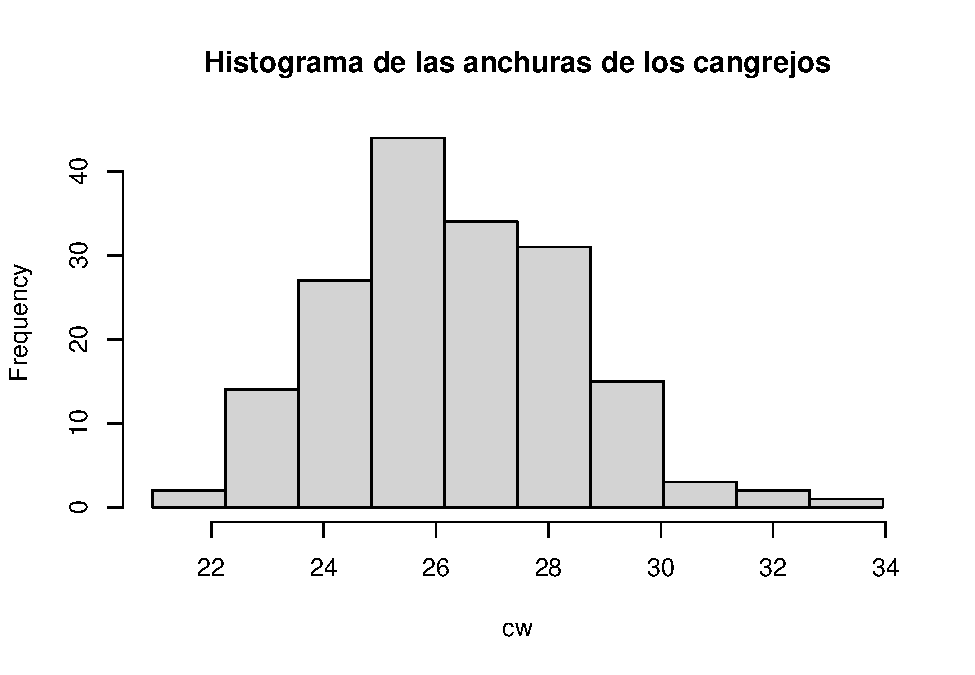
\includegraphics{EstadisticosAgrupados_files/figure-latex/unnamed-chunk-7-1.pdf}

\begin{Shaded}
\begin{Highlighting}[]
\CommentTok{\#Mirando la estrucutra interna, con plot = F}
\FunctionTok{hist}\NormalTok{(cw, }\AttributeTok{breaks =}\NormalTok{ L, }\AttributeTok{right =}\NormalTok{ F, }\AttributeTok{plot =}\NormalTok{ F)}
\end{Highlighting}
\end{Shaded}

\begin{verbatim}
## $breaks
##  [1] 20.95 22.25 23.55 24.85 26.15 27.45 28.75 30.05 31.35 32.65 33.95
## 
## $counts
##  [1]  2 14 27 44 34 31 15  3  2  1
## 
## $density
##  [1] 0.008892841 0.062249889 0.120053357 0.195642508 0.151178301 0.137839040
##  [7] 0.066696309 0.013339262 0.008892841 0.004446421
## 
## $mids
##  [1] 21.6 22.9 24.2 25.5 26.8 28.1 29.4 30.7 32.0 33.3
## 
## $xname
## [1] "cw"
## 
## $equidist
## [1] TRUE
## 
## attr(,"class")
## [1] "histogram"
\end{verbatim}

\begin{Shaded}
\begin{Highlighting}[]
\CommentTok{\#Usando las funciones preparadas, primero absoluta, luego absoluta acumulada}
\FunctionTok{histAbs}\NormalTok{(cw, L)}
\end{Highlighting}
\end{Shaded}

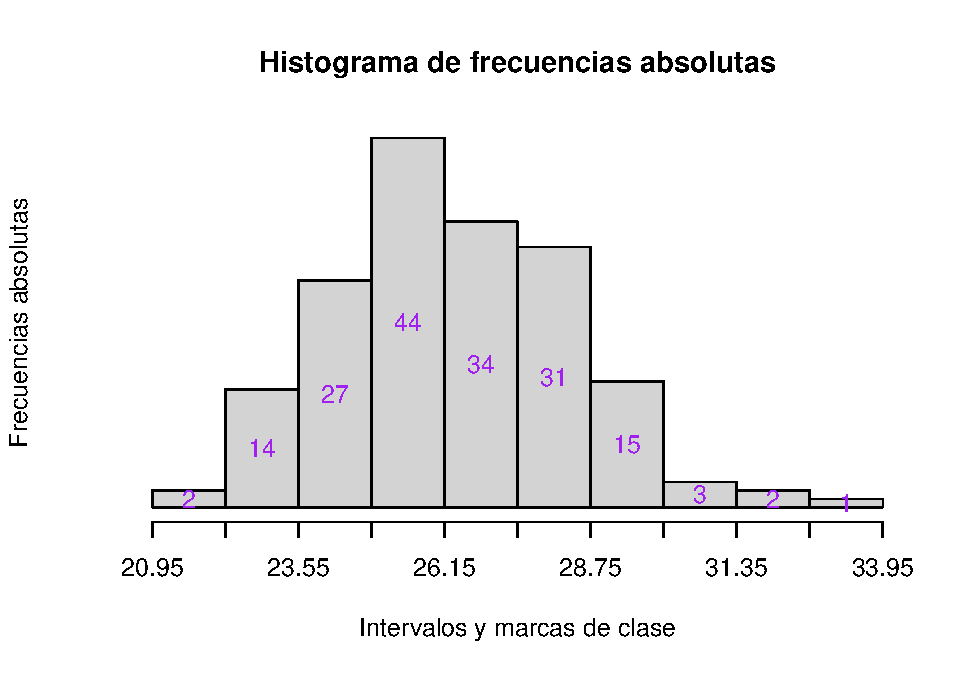
\includegraphics{EstadisticosAgrupados_files/figure-latex/unnamed-chunk-7-2.pdf}

\begin{Shaded}
\begin{Highlighting}[]
\FunctionTok{histAbsCum}\NormalTok{(cw, L)}
\end{Highlighting}
\end{Shaded}

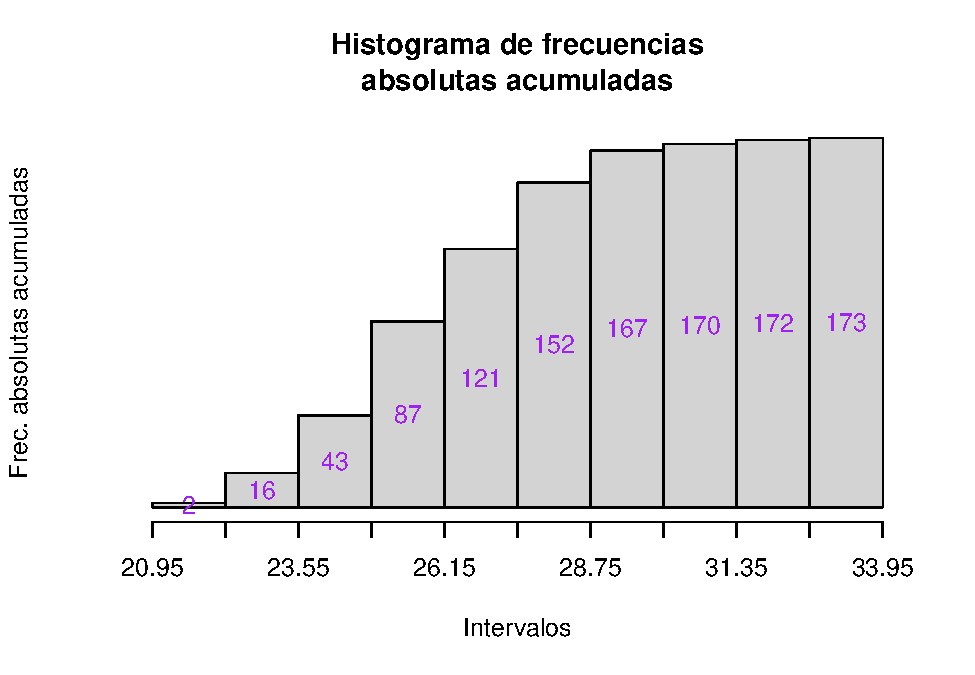
\includegraphics{EstadisticosAgrupados_files/figure-latex/unnamed-chunk-7-3.pdf}

\end{document}
